\let\textcircled=\pgftextcircled
\chapter{Interface Design}
\begin{figure}
\begin{center}
\begin{tabular}{cc}
\subfloat{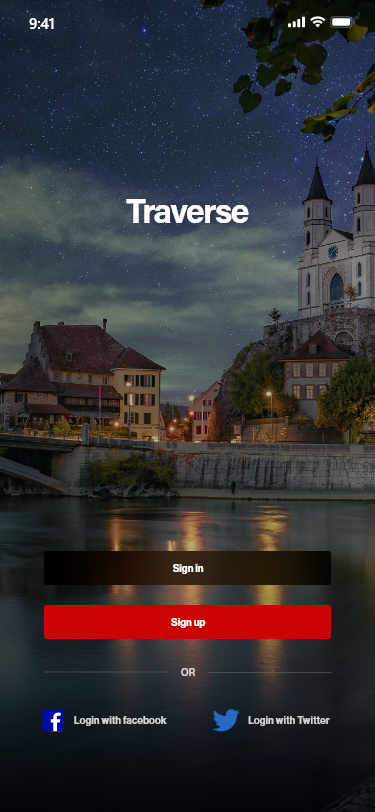
\includegraphics[height = 0.5\textheight]{Exports/land.png}} &
\subfloat{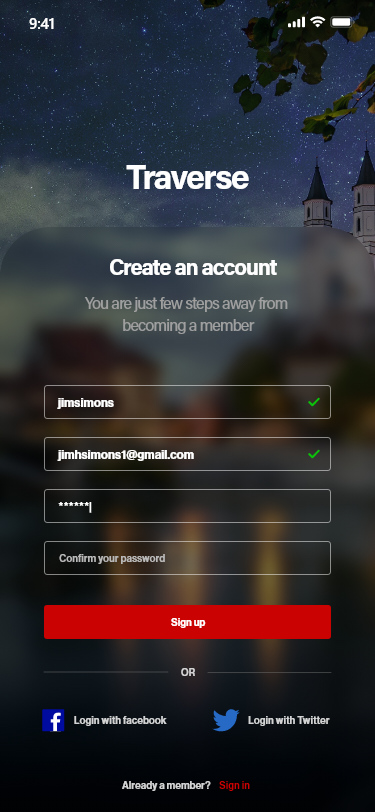
\includegraphics[height = 0.5\textheight]{Exports/su.png}} \\
\subfloat{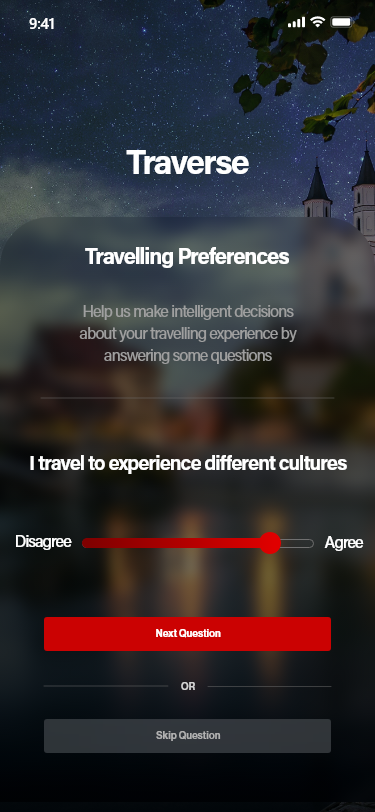
\includegraphics[height = 0.5\textheight]{Exports/pref.png}} &
\subfloat{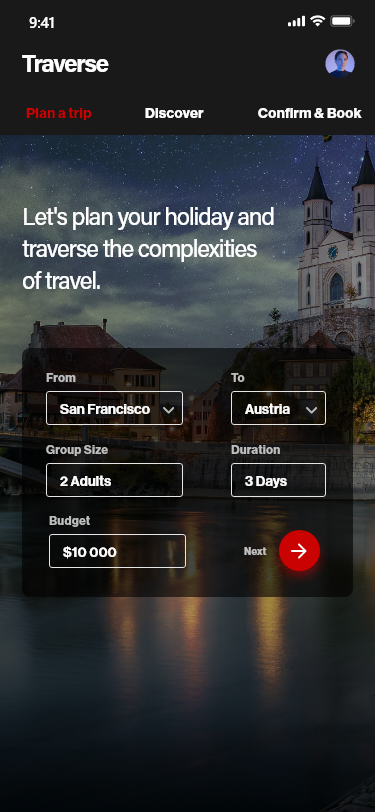
\includegraphics[height = 0.5\textheight]{Exports/mli.png}}
\end{tabular}
\end{center}
\end{figure}
\begin{figure}
\begin{center}
\begin{tabular}{cc}
	\subfloat{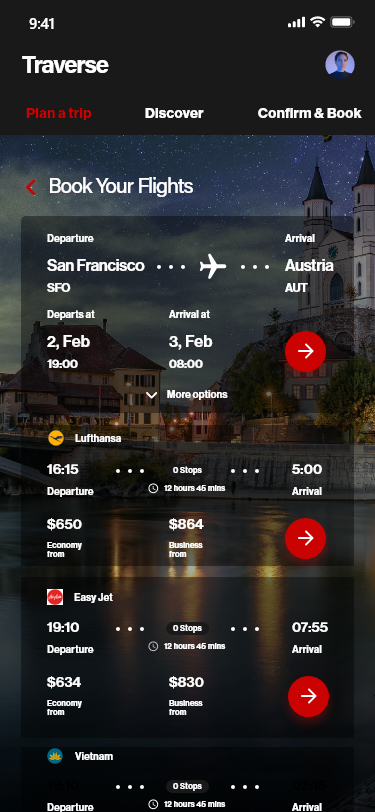
\includegraphics[height = 0.5\textheight]{Exports/fli.png}} &
\subfloat{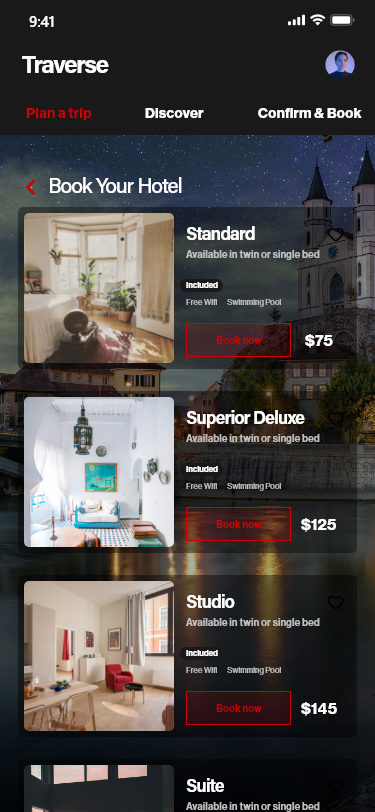
\includegraphics[height = 0.5\textheight]{Exports/hot.png}} \\
	\subfloat{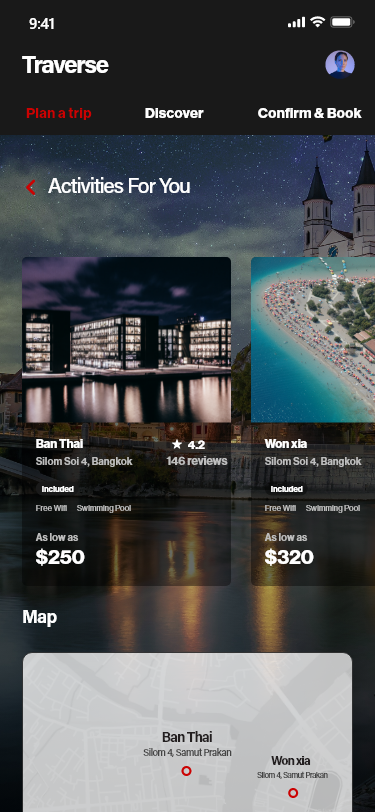
\includegraphics[height = 0.5\textheight]{Exports/act.png}} &
\subfloat{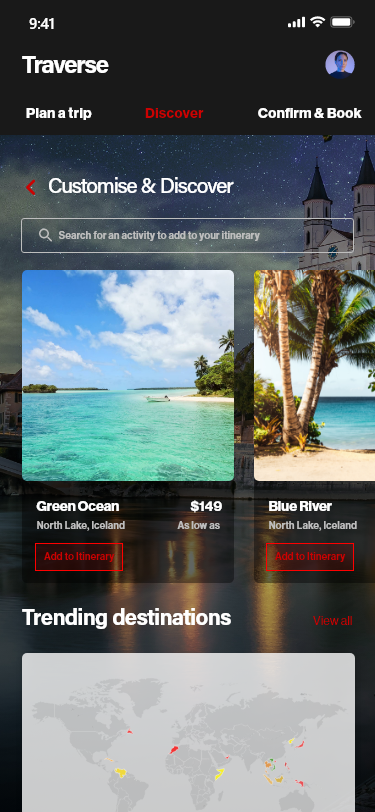
\includegraphics[height = 0.5\textheight]{Exports/dis.png}} 
\end{tabular}
\end{center}
\end{figure}
\begin{figure}
\begin{center}
\begin{tabular}{cc}
\subfloat{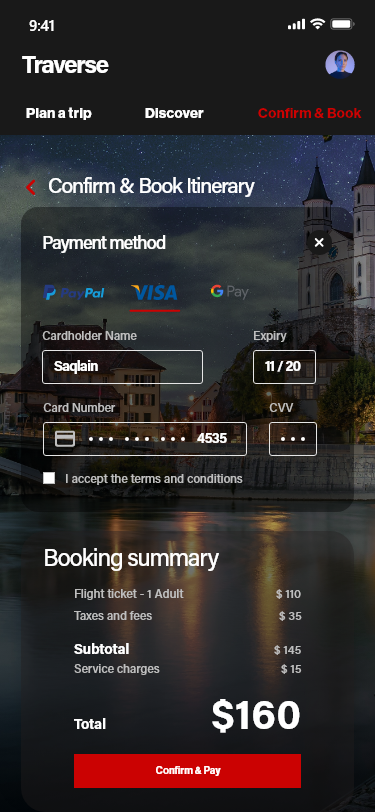
\includegraphics[height = 0.5\textheight]{Exports/pay.png}} &
\subfloat{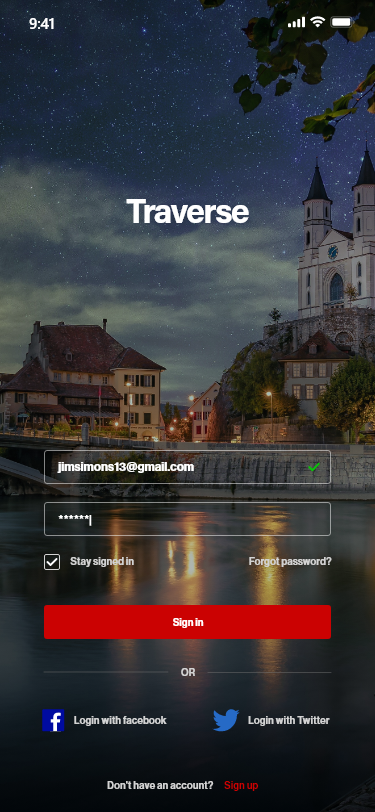
\includegraphics[height = 0.5\textheight]{Exports/si.png}} \\
\subfloat{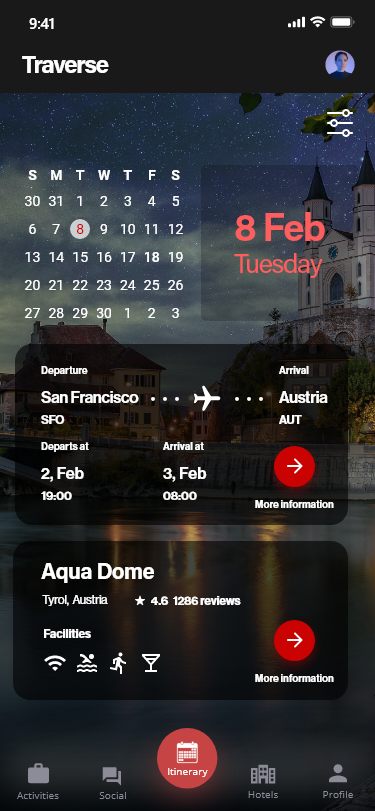
\includegraphics[height = 0.5\textheight]{Exports/main.png}} & 
\subfloat{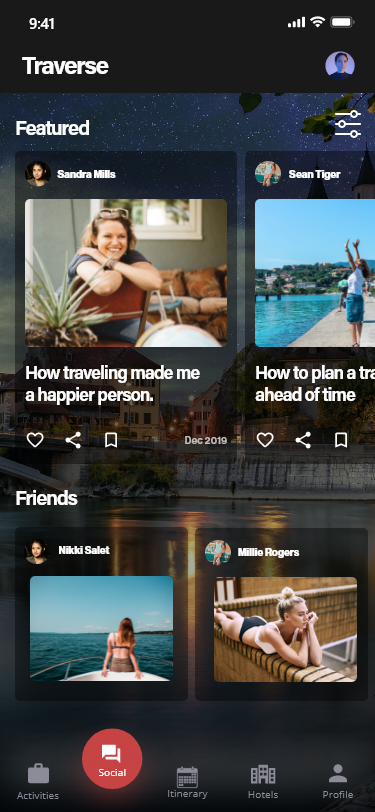
\includegraphics[height = 0.5\textheight]{Exports/soc.png}} 
\end{tabular}
\end{center}
\end{figure}


